\documentclass[journal,a4paper]{IEEEtran}

% IEEE-style report;
\usepackage[T1]{fontenc}
\usepackage{amsmath,amsfonts,amssymb,amsthm}
\usepackage{graphicx}
\usepackage{url}
\usepackage[numbers,sort&compress]{natbib}
\usepackage{hyperref}
\usepackage{booktabs}
\usepackage{tabularx}
\usepackage{array}
\usepackage{tikz}
\usetikzlibrary{arrows.meta,positioning,calc}
\usepackage{enumitem}
\usepackage{microtype}
\usepackage{comment}
\usepackage{float}

\hypersetup{colorlinks=true, linkcolor=black, urlcolor=blue, citecolor=black}
\setlist[itemize]{leftmargin=1.2em, itemsep=1pt, topsep=2pt}
\setlist[enumerate]{leftmargin=1.4em, itemsep=1pt, topsep=2pt}
\newcommand{\dd}{\,\mathrm{d}}
\newcommand{\sat}{\operatorname{sat}}
\newcommand{\wrap}{\operatorname{wrap}}

\begin{document}

\title{Closed-Loop Acoustic Tracking of a Moving Rover for Real-Time Localization}

\author{Helene~Jabbour}

\markboth{MECH 653 / EECE 660: System Analysis and Design --- Progress Report}{Jabbour and Raffoul: Acoustic Rover Pursuit}

\maketitle

% Abstract (IEEEtran formats the heading and bolding natively)
\begin{abstract}
This project investigates acoustic localization and closed-loop pursuit of a moving target using a low-cost mobile robot. A follower rover equipped with a MAX4466 microphone inside a 3D-printed directional horn estimates the relative position of a target rover emitting a known acoustic signal. A measurement model and a local linearized state-space model are proposed. The remaining work includes validating the models, analyzing stability, controllability, and observability, and designing and testing a feedback controller. The intended outcome is an experimental demonstration of acoustic-guided rover pursuit, supported by simulation results and an associated codebase.
\end{abstract}

% IEEE Keywords Block
\begin{IEEEkeywords}
Acoustic tracking, bearing-only pursuit, state-space modeling, feedback control, embedded systems.
\end{IEEEkeywords}

\section{Introduction and Motivation}
\IEEEPARstart{I}{n} robot rendezvous and pursuit problems, a robot must locate and meet another robot with unknown relative position within a finite time \cite{lin2003}. Such problems arise in applications like emergency response, wildlife tracking or space exploration, where an autonomous robot needs to follow or locate the target with limited access to visual information or positioning systems. The tracking challenge often appears in research areas such as robotic sound-source localization that investigates how robots can locate acoustic sources, mobile robots that use rotating antennas to track radio-tagged wildlife, and bearing-only sonar research \cite{rascon2017review,tokekar2011active,nardone1981observability,lingren1978position}. Across these applications with different sensing modalities, the common challenge consists of converting the measurements into sufficiently reliable estimates of the target's relative state and using them as feedback to guide the follower's motion.

This project investigates real-time feedback control for an autonomous rover tracking a moving acoustic beacon with no access to the target's position or velocity. The ``target" rover follows an open-loop trajectory while repeatedly emitting an acoustic beacon through an on-board Bluetooth speaker, while the ``follower" rover uses a MAX4466 microphone mounted inside a 3D-printed horn (in order to make the sensor directional) rotated by a servo motor fixed on the rover. The horn is continuously sweeping to measure signal intensity and uses the received signals to estimate the relative position of the target. The follower is actuated and steered to approach the target and remain within a fixed distance of it.

A preliminary proof of concept (Appendix  \ref{app:poc}) is completed to compare sound signal from various distances and orientations using an ESP32, a MAX4466 microphone, and a speaker -- both with and without the directional horn. Building on these results along with a review of the existing literature, a dynamic LTI state-space model is derived and the control objectives are established. Once system analysis and design are conducted, the proposed controller will be simulated then tested on the physical rovers. The project focuses on planar indoor motion on a flat floor with relative localization and within a distance of a few meters.

The research question is therefore: \textbf{To what extent can a low-cost acoustic sensing system enable a mobile robot to follow a moving target, and how accurately can the local LTI model predict system dynamics?}

\section{Literature Review}
\subsection{Sound Source Localization}

The first part of the proposed project (before the motion control itself) involves deducing the target's position by sensing its acoustic transmissions. Sound Source Localization (SSL) is a mature field from which the project can borrow heavily. \citet{rascon2017review} and
\citet{argentieri2015survey} both conducted extensive reviews on SSL methods.

\citet{rascon2017review} mostly look at strategies used by arrays of omnidirectional microphones (usually 2) to locate one or multiple sound sources. The main strategy across papers for angle estimation is to process the received signal to extract certain statistics, use a grid search or a trained model to map these statistics to a location, then to smooth the result via different filters (depending on the specific setup). Distance estimation is more tricky: the extracted signal statistics correlates more weakly with source distance compared to source angle, especially when the source's baseline loudness is unknown or multiple sources are transmitting at once. Some surveyed works choose to leverage robot movement to resolve this (which is the approach most relevant to our setup), by triangulating using measurements taken from different positions, sometimes explicitly moving the robot closer to the source. 

\citet{argentieri2015survey} look separately at binaural methods (which use two
microphones to imitate human hearing) and array methods (more than 2 microphones). Binaural
systems rely on the interaural time and level differences (intensity is limited in usefulness when the source's loudness is unknown). Array methods use a variety of techniques such as beamforming (which shifts each microphone’s signal by the delays a candidate direction predicts and keeps the direction that results in the highest array energy), Generalized Cross-Correlation with Phase Transform (GCC-PHAT), or Multiple Signal Classification (MUSIC).
Array methods are found to be overall more robust, and the review stresses the under-utilization of robot motion in SSL (what is called \emph{active audition} \cite{nakadai2000active}). Several techniques can leverage active audition to refine estimates, for example by intersecting successive ``cones of confusion'' (the set of directions consistent with the measurements at each position).

The closest application in SSL is found in the work of
\citet{luo2010docking}. They built an indoor robot that finds a sound-emitting charging dock using two microphone pairs, a camera and laser scanner.

\subsection{Rotating Sensor Arrays and Leveraging Robot Motion}

The specific strategy of rotating a directional sensor and using its amplitude readings to deduce source location is well-established, although it is more commonly found in radio applications. \citet{graefenstein2009wireless} are an early example of the setup, using a rotating directional antenna on a ground robot to estimate the angle of arrival (AoA) of a wireless node from the detected signal strength during the rotation.

There is significant design freedom in how exactly each sweep becomes a direction estimate. There is no consensus, and methods range from simple heuristics to more involved estimates: \citet{graefenstein2009wireless}
take the angle of strongest signal (a natural choice); \citet{venkateswaran2013rf} split the angular space into bins and average the readings within each to extract the loudest bin; \citet{tokekar2011active} sample the signal strength at
fixed angles and fit a polynomial around the maximum. Some methods take advantage of the whole sweep rather than discarding most readings: \citet{singleantenna2025} model the antenna's known radiation pattern to derive a maximum-likelihood (ML) angle estimator; the resulting estimated angle is the one most likely to produce the intensity reading observed over the whole sweep (which might not happen to align with the angle of strongest signal if the other, less loud directions give contradictory information).

Once an angle is deduced from a sweep (in whatever way is previously chosen), there is further design freedom in how to use this estimate. A heuristic greedy strategy that circumvents the need for explicit target location estimation is to follow the estimated direction until a new sweep is completed and the angle is updated; we see it applied in the work of \citet{venkateswaran2013rf} who mount a directional
antenna on a naturally spinning micro aerial vehicle. They show that, given some bounds on the noise and frequency of outliers, the vehicle returns to a small ball around the source (whose radius grows with the distance traveled between each sweep) infinitely often. The strategy proves remarkably robust to the error of individual estimates: 23\% of
the bearings were off by more than $60^\circ$, yet a rover was able to reach a source initially 55\,m away in only 59.9\,m of flight, the large angle errors canceling out over the course of the run. 

The more involved way is to actually estimate source position and refine this estimate with each sweep. This strategy can sometimes interfere with robot motion: there is incentive in moving the robot to a ``good measurement spot", a spot that produces new information and allows the location estimate to converge quickly. This movement goal might not necessarily contribute to bringing the robot closer to the source, and there is a tradeoff between minimizing unnecessary movement on the path to the source and exploiting robot motion to get varied and useful measurement. \citet{feldbaum1960dual} calls this the dual effect of control, and optimal dual control is not generally tractable.

\citet{deghat2014localization} explicitly frame their estimator\textbackslash controller design task as dual control. In their setup, the observer must estimate the location of a target (which may drift slowly), then it must circle it at a given radius. Their estimator corrects the error perpendicular to the bearing while the controller moves closer to the target (sideways, in order to always rotate the bearing). They prove that the estimation error converges exponentially if and only if the bearing keeps sweeping through all directions (\emph{persistence of excitation}, a condition that circling the target guarantees).

Wildlife-tracking literature, where robots locate radio-tagged animals, provides many useful examples of dual control. \citet{tokekar2011active} use a ground robot equipped with a rotating directional antenna to locate invasive fish under lake ice, choosing sensing locations to minimize the
uncertainty of the estimate. 

\citet{vanderhook2014cautious} minimize
the total time spent traveling and measuring, landing on a ``cautious greedy'' strategy. Briefly, the target's position is estimated with an extended Kalman filter (EKF) whose uncertainty looks like an ellipse around the current estimate. At each step, the robot moves to a point
from which its line of sight to the estimate is perpendicular to the long axis of the uncertainty ellipse (this is the direction in which the target's position is least known), so that each new bearing reduces the largest uncertainty. It also stays far enough from the current estimate that the target
is unlikely to be behind it (to minimize the effect of the antenna's front--back ambiguity). Since this safe distance shrinks with the uncertainty, the robot effectively zigzags towards the targets as it locates it, meaning locating and approaching happen along the same path. The strategy is shown to be within a constant factor of the best achievable (time-wise). A cone with a single opening (i.e. without front--back ambiguity) performs even better, although reflections can still produce misleading
spurious peaks.
\citet{vanderhook2015algorithms} extend the analysis to several robots under communication constraints.

\citet{chen2023conservationbots} track several animals with an aerial robot and combine angle of arrival (AoA) and received signal strength indicator (RSSI) methods. They design a planner that jointly decides where to fly and which type of measurement to take (angle or strength), and note the effect of target motion on that choice: sensor rotations, which are slow to perform, are more accurate for static animals but become
counterproductive when the target moves.

The main takeaway here is that a single bearing only constrains the source to a line, and it is the sensor's motion between
measurements that pins down its exact position. The literature on submarine sonars can be surprisingly informative in determining what makes this motion ``useful" (from the point of view of maximizing information extracted from measurements). 

\citet{lingren1978position} analyzed whether the position and velocity of a target ship can be deduced by the bearing measurements of an observer ship, and \citet{nardone1981observability} gave
necessary and sufficient conditions on the observer's motion for a constant-velocity target. They conclude that a constant-velocity observer cannot always determine a constant-velocity target (acceleration is necessary), and that motion along the line of sight is not sufficient (even in the presence of observer acceleration). For a stationary source, two bearings that do not lie on the line of sight are sufficient. 
While the rover in our setup has access to intensity readings (unlike the ships in this analysis), the literature on submarine sonar supports the usefulness of occasionally leaving the line of sight path (the shortest path to the source) in order to gain confidence in the location estimate. This is reminiscent of the zigzag cautious greedy strategy of \citet{vanderhook2014cautious}.


\subsection{Estimating the Target Position}

The estimators relevant to our setup are approximations of the recursive Bayes filter, which, at each step, predicts the target position given its internal model of the problem dynamics then updates its belief with each new measurement depending on how much they align with the prediction (i.e. depending on the conditional probability of receiving the measurement given the current belief about the target location). \citet{thrun2005probabilistic}, \citet{barshalom2001estimation}, and \citet{simon2006optimal} derive various useful models for different estimation scenarios.

The main filters of interest mostly differ in the way they model belief about the target position: the Kalman filter \citep{kalman1960new} is for linear models; the Extended Kalman Filter (EKF) tolerates nonlinear models by linearizing them around the current estimate; the Unscented Kalman Filter (UKF) \citep{julier2004unscented} propagates a small set of sample points through the nonlinear model (rather than linearizing it); particle filters \citep{gordon1993novel,arulampalam2002tutorial} represent their belief about target location as weighted samples (each sample being a hypothesis), which makes them able to keep track of several strong candidates until the uncertainty is resolved (a relevant feature in the case of very strong reflections for instance); and grid filters break the map into cells and store for each cell the probability that the target is located in it.

\citet{aidala1983utilization} show that a Cartesian-coordinate EKF in a bearing-only setup can become overconfident and diverge, and propose the use of modified polar coordinates to separate observable (without the need for motion) quantities (like bearing) from the unobservable (requiring observer motion) ones (like range). \citet{ristic2004beyond} compare the EKF, the UKF, and particle filters on bearing-only tracking.


\subsection{Control of a Differential-Drive Rover}
The chosen observer is a differential-drive rover, and strategies for controlling it are well-established, usually via Model predictive control (MPC)
\citep{mayne2000constrained,rawlings2017model}. Different strategies specific to a moving target also exist (i.e. ways to reach it more efficiently than simply aiming for its current position) \citep{zarchan2012tactical,deghat2014localization,shames2012circumnavigation}. We do not expand much on this aspect of the control at the present time due to length constraints.

\subsection{Summary and Literature Gap}
Overall, there is significant work on Sound Source Localization, leveraging rotating sensors and robot motion for location estimation, and dual control. The dynamics of differential-drive rovers are also well understood (although skipped). The specific setup remains unique, especially given the choice of acoustic waves (as opposed to radio), and the many degrees of freedom in the design of the estimator and controller (the use of an estimator at all being itself a choice) mean that many specific combinations have not been validated.


\section{System Description}
\label{sec:system}

\subsection{Hardware Description}
The setup consists on two SunFounder PiCar-S vehicles  (\autoref{fig:cars}). The Raspberry Pi of the target implements an open-loop motion script while the on-board Bluetooth speaker emits a software-driven burst sound with constant volume and frequency  $f_0$ at regular intervals. 

On the follower, a MAX4466 microphone (electret microphone amplifier with adjustable gain) \cite{mic} provides an analog audio waveform. It is mounted at the back of a 3D-printed PLA-based horn fixed to an SG90 servo motor placed on the follower rover (\autoref{fig:cars}). Using a directional horn is essential to the setup to consolidate sound capture into one identifiable range of sight (sound). However, audio signal acquisition requires external ADC sampling as Raspberry Pi has no analog input. Therefore, an ESP32 microcontroller executes signal sampling; it also computes and sends the acoustic features to the follower Raspberry Pi over USB serial, and it controls the servo rotation. The Raspberry Pi then runs the proposed controller and commands the vehicle's steering and speed. 

\begin{figure}[ht!]
\begin{center}
    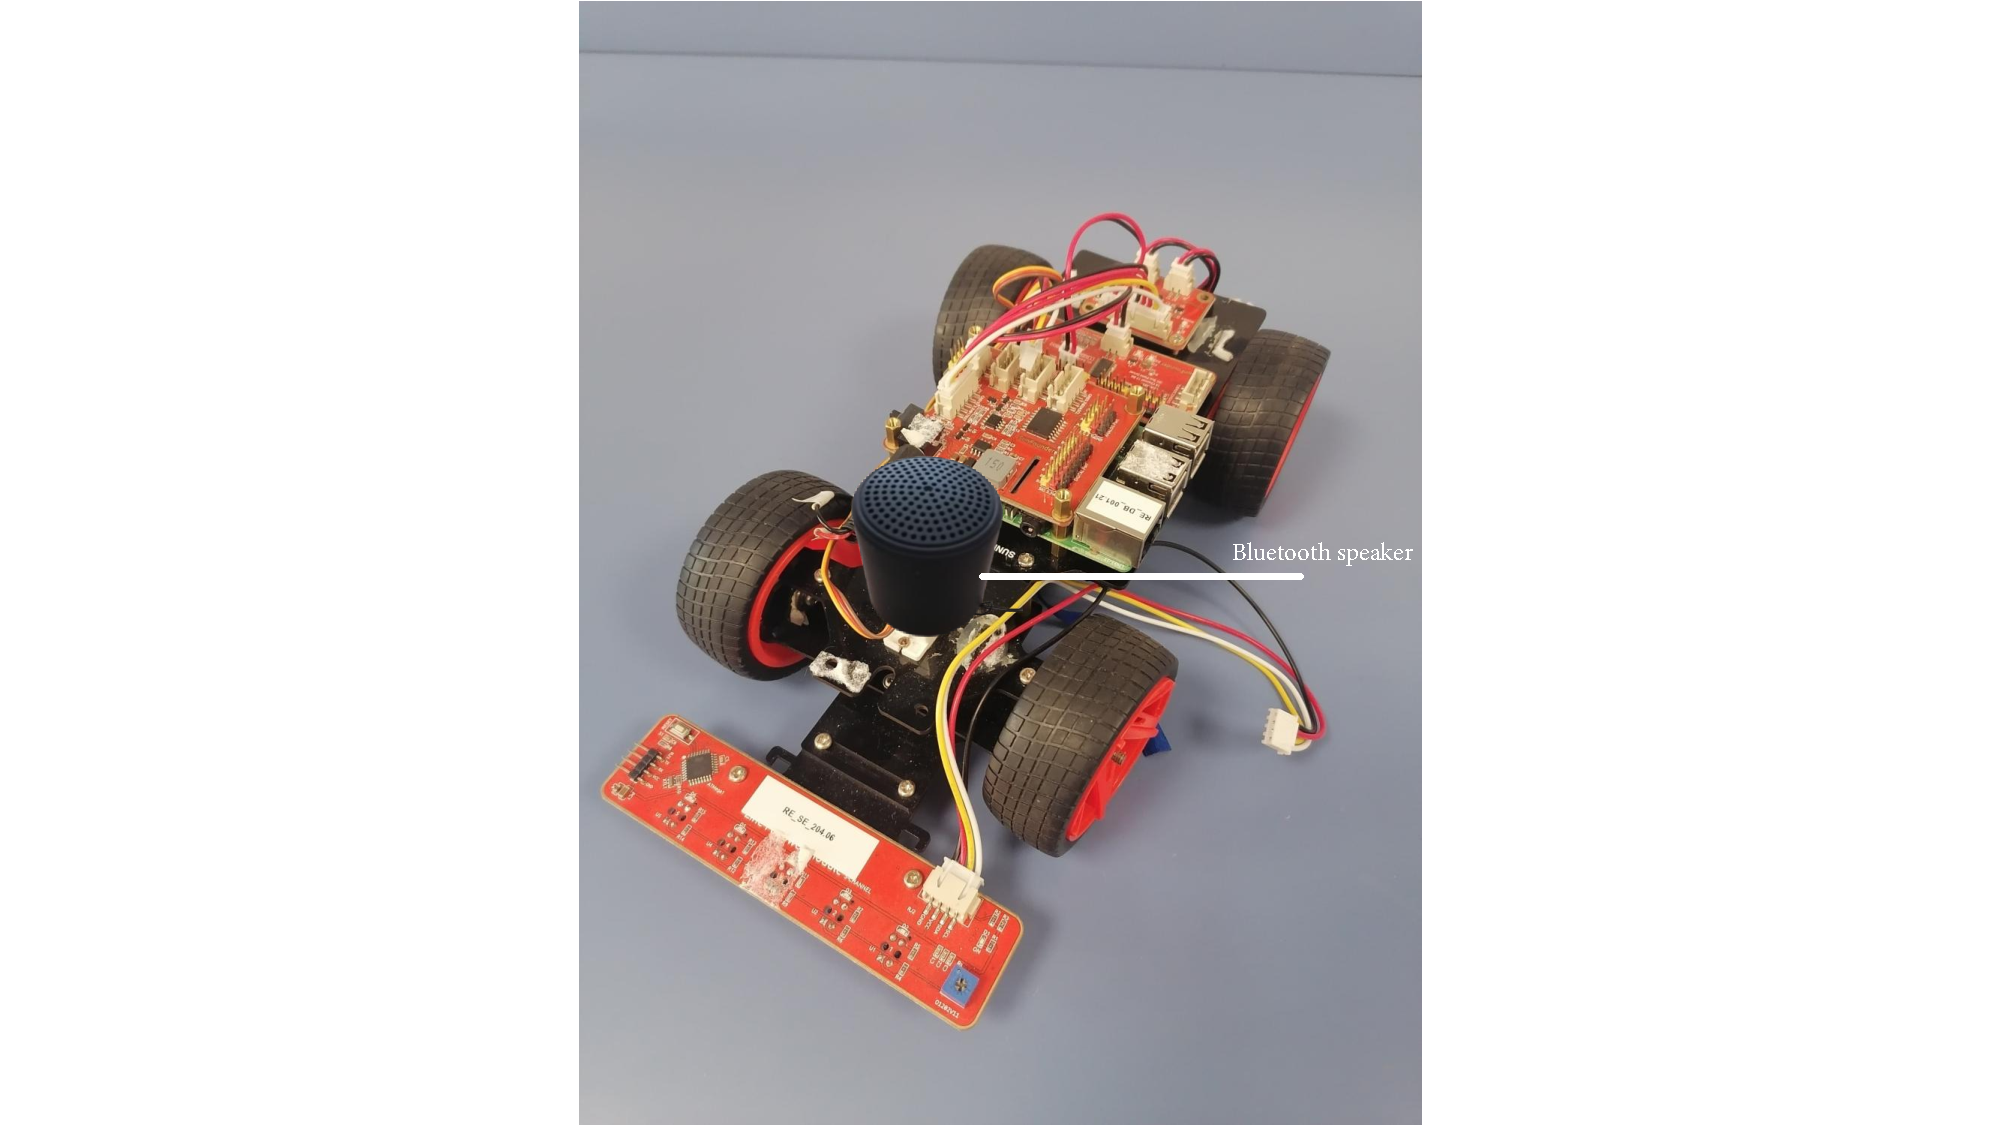
\includegraphics[width=0.43\linewidth]{target_horn.pdf}
    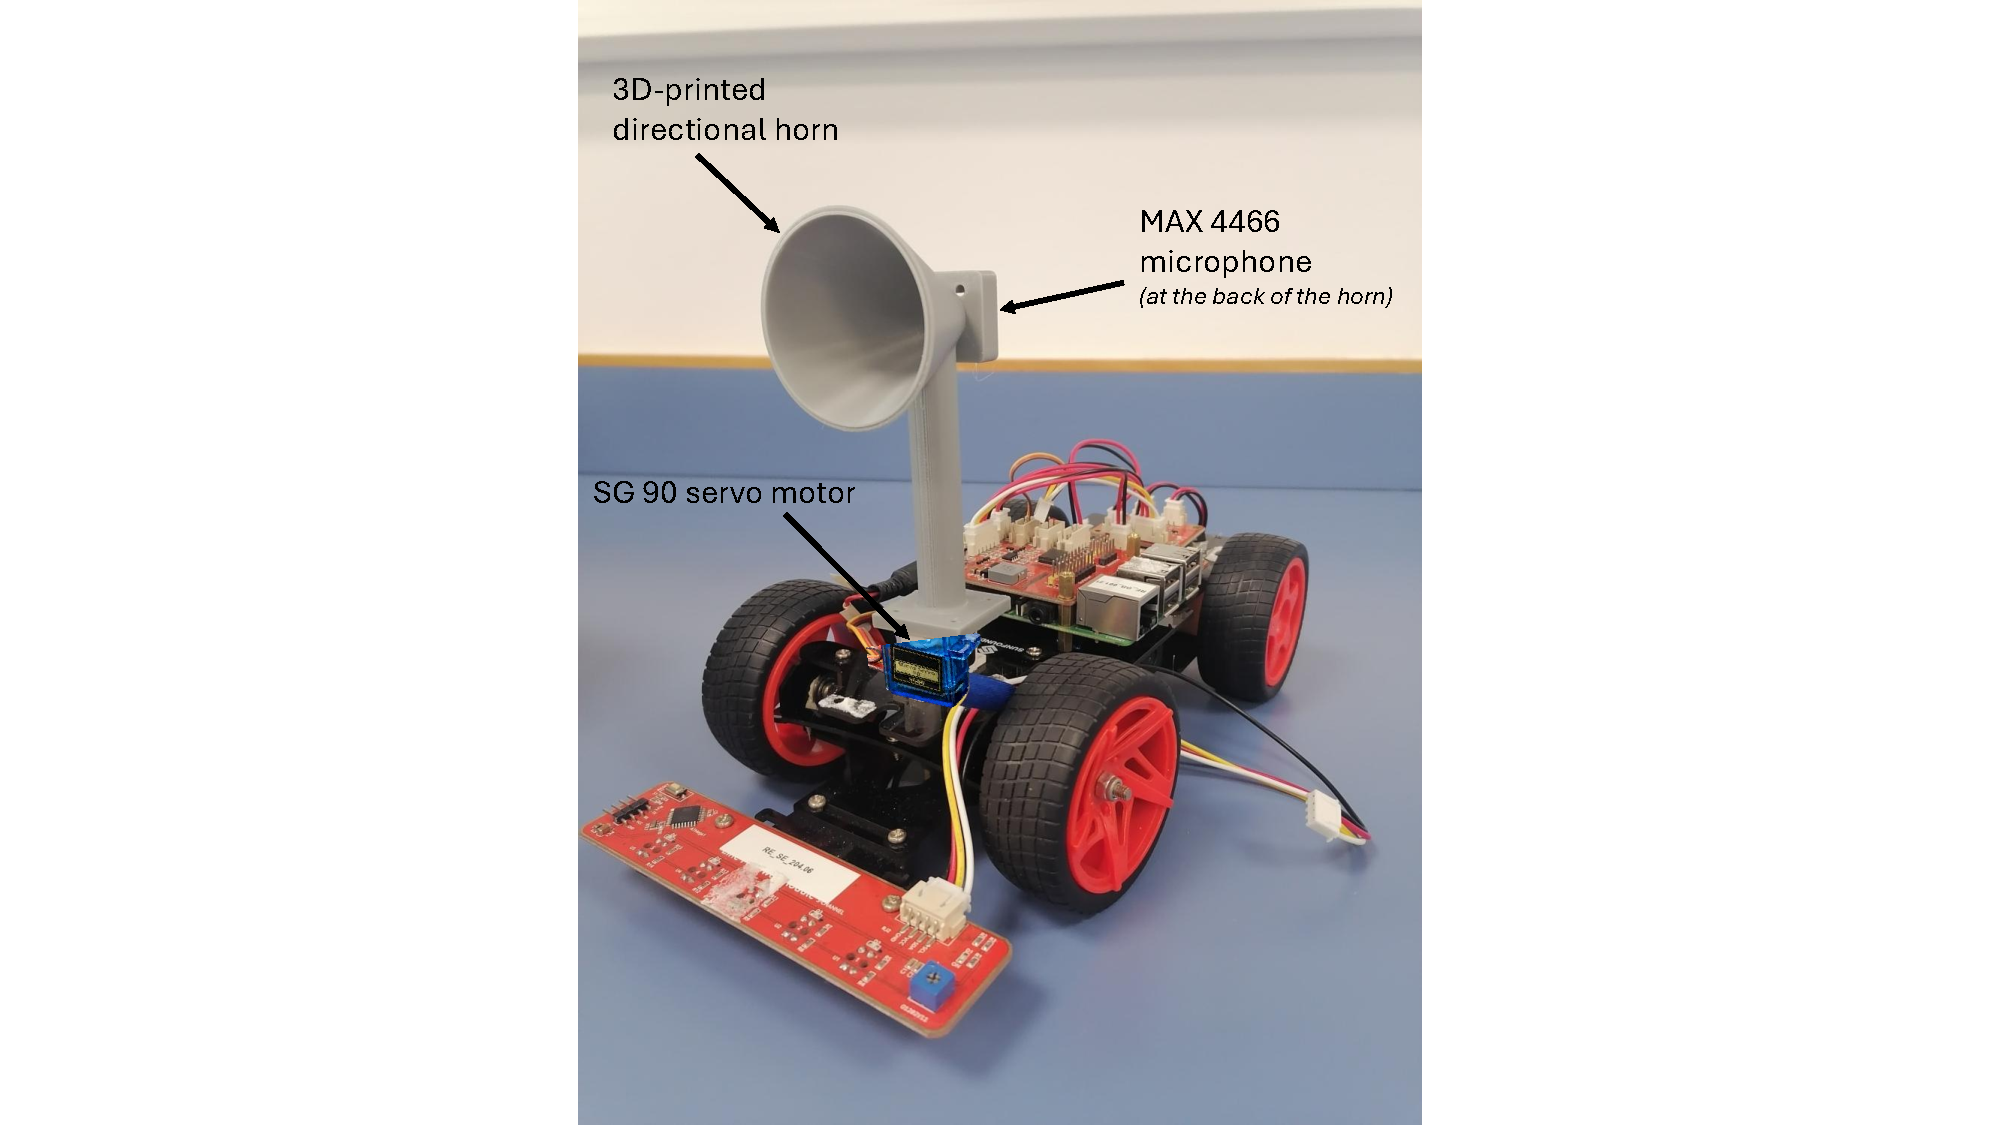
\includegraphics[width=0.43\linewidth]{follower.pdf}
    \caption{"Target" SunFounder PiCar-S with mounted Bluetooth speaker (left) and "Follower" SunFounder PiCar-S with 3D-printed directional horn housing MAX4466 microphone (right).}
    \label{fig:cars}
\end{center}
\end{figure}

\subsection{System Architecture}

The system architecture has four stages: acquire the beacon, estimate its relative bearing, steer and advance, and stop when the near-target condition is reached. 

In the initial sensing phase, the horn sweeps between two orientations, $\varphi_c-\delta$ and $\varphi_c+\delta$, to detect the beacon, where $\varphi_c$ denotes the arm's pointing angle measured relative to the follower's forward direction, and $\delta$ is the sweep angle. This local scan runs continuously, with a wider scan reserved for signal loss. ESP32 then estimates the corresponding sound wave amplitudes $A_-$ and $A_+$ (\autoref{eq:amp}) and runs a signal quality validation before sending them, along with timestamps, to the Raspberry Pi. A USB link carries one packet $(t,\varphi_c,A_\pm)$ per measurement. 

Subsequently, on the Raspberry Pi, the acoustic data is converted into relative range (i.e., distance between two rovers) estimate $\hat{\rho}$ (\autoref{eq:rho}) and bearing (i.e., angle of the target measured relative to the follower’s forward direction) estimate $\hat{\beta}$ (\autoref{eq:beta}). \autoref{fig:geom} clarifies the space geometry considered. A state observer propagates the state estimate at the control rate $f_c$ and corrects it with new sound measurements. 

A state-feedback controller computes the follower's speed and yaw-rate commands at the rate of $f_c$ (rate to be determined via testing). The horn pointing reference is updated according to $\varphi_c=\hat{\beta}$ (subject to the mechanical limits of the servo) so that the sensor captures a new measurement in the target's estimated direction.

In the scenario where the beacon is lost or the measurements become invalid, the follower reduces or stops its forward motion and initiates a new acquisition after a specified timeout. The control model is developed around a local straight-line operating condition; acquisition and reacquisition are treated as supervisory functions rather than as part of the linearized controller.

The software used consists of Python on the Pi and a Windows PC, and MATLAB/Simulink for design and simulation.

\autoref{fig:arch} summarizes the overall sensing, acquisition, and control architecture. 

\begin{figure}[!t]
\centering
\resizebox{\linewidth}{!}{%
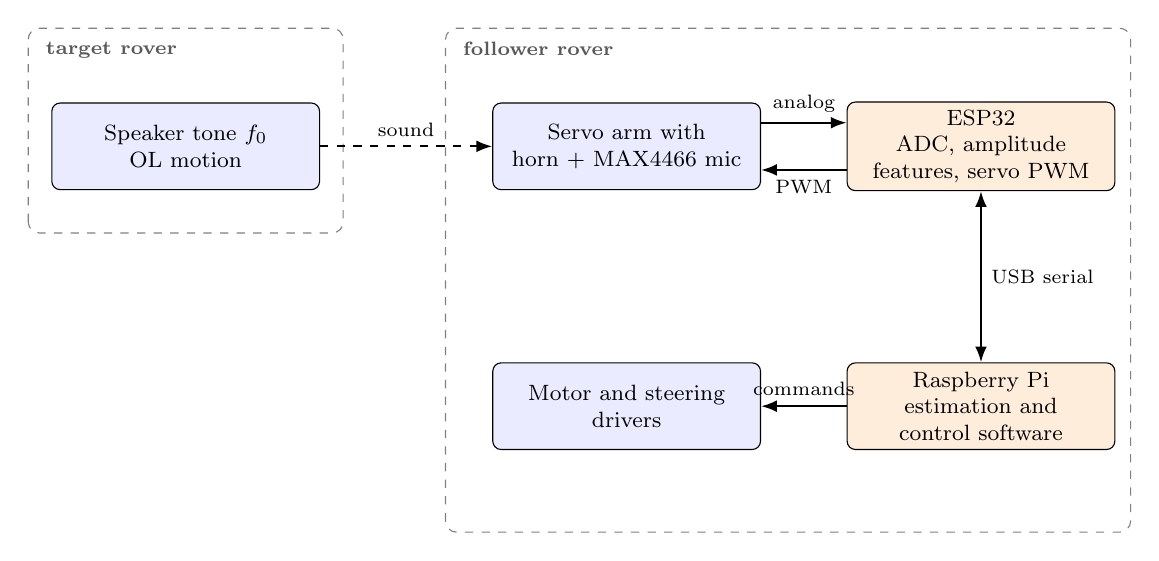
\begin{tikzpicture}[
  font=\footnotesize,
  blk/.style={draw, rounded corners=3pt, align=center, minimum height=11mm, minimum width=34mm, inner sep=3pt},
  hw/.style={blk, fill=blue!8},
  sw/.style={blk, fill=orange!14},
  link/.style={-{Latex[length=2mm]}, thick},
  both/.style={{Latex[length=2mm]}-{Latex[length=2mm]}, thick},
  snd/.style={-{Latex[length=2mm]}, thick, dashed},
  lbl/.style={font=\scriptsize, align=center},
  box/.style={draw, dashed, rounded corners=4pt, gray}
]
% ---- rover containers
\draw[box] (-0.4,-1.1) rectangle (3.6,1.5);
\node[lbl, anchor=north west, gray!70!black] at (-0.3,1.45) {\textbf{target rover}};
\draw[box] (4.9,-4.9) rectangle (13.6,1.5);
\node[lbl, anchor=north west, gray!70!black] at (5.0,1.45) {\textbf{follower rover}};
% ---- components
\node[hw] (tgt) at (1.6,0) {Speaker tone $f_0$\\OL motion};
\node[hw] (mic) at (7.2,0) {Servo arm with\\horn + MAX4466 mic};
\node[sw] (esp) at (11.7,0) {ESP32\\ADC, amplitude\\features, servo PWM};
\node[sw] (pi)  at (11.7,-3.3) {Raspberry Pi\\estimation and\\control software};
\node[hw] (drv) at (7.2,-3.3) {Motor and steering\\drivers};

% ---- links
\draw[snd] (tgt.east) -- node[above, lbl] {sound} (mic.west);
\draw[link] ([yshift=3mm]mic.east) -- node[above, lbl] {analog} ([yshift=3mm]esp.west);
\draw[link] ([yshift=-3mm]esp.west) -- node[below, lbl] {PWM} ([yshift=-3mm]mic.east);
\draw[both] (esp.south) -- node[right, lbl] {USB serial} (pi.north);
\draw[link] (pi.west) -- node[above, lbl] {commands} (drv.east);
\end{tikzpicture}%
}
\caption{System architecture: hardware components and communication links. Blue: physical elements; orange: computation. The signals and the control loop are shown in Fig.~\ref{fig:ctrl}.}
\label{fig:arch}
\end{figure}


\section{Measurement Model and State-Space Model}
\subsection{Acoustic Sensing Model}
\label{sec:sensing}
The ESP32 samples the analog output of the MAX4466 microphone and estimates the acoustic amplitude using a Goertzel filter \cite{goertzel} (using Discrete Fourier Transform) over $N$ samples:
\begin{equation}
A=
\frac{2}{N}
\left|
\sum_{n=0}^{N-1}
s[n]e^{-j2\pi f_0 n/f_s}
\right|,
\label{eq:goertzel}
\end{equation}
where $f_s$ is the sampling frequency and $s[n]$ denotes the mean-removed ADC samples. The tone frequency $f_0$, sampling rate $f_s$, and window length will be selected from testing. It is ensured that the two amplitudes $A_-$ and $A_+$ are acquired close enough in time so that variations in the target's motion do not invalidate the paired-measurement assumption.

An expression of the acoustic amplitude $A$ as a function of the range ${\rho}$, arm angle $\varphi$, and bearing ${\beta}$ is derived. $A$ is assumed to be inversely proportional to the range ${\rho}$. The horn adds a directional gain $G(\Delta)$, where $\Delta=\varphi-\beta$ is the pointing error between the arm angle $\varphi$
and the target bearing $\beta$ (both relative to the follower's heading), and
$G(0)=1$. Hence
\begin{equation}
A(\varphi)=\frac{K}{\rho}\,G(\varphi-\beta)+n,\qquad
G(\Delta)\approx e^{-\Delta^{2}/(2\sigma^{2})}.
\label{eq:amp}
\end{equation}
$n$ is measurement noise. $G$ depends on the horn geometry and follows a Gaussian with parameters $\sigma$ and $\Delta$. These parameters will be estimated using calibration, i.e., $\sigma$ from angular sweeps and $K$ from measurements at different distances.

Assuming that the target range ${\rho}$ remains constant during the paired measurements $A_-$ and $A_+$ at $\varphi_c-\delta$ and $\varphi_c+\delta$, respectively, the bearing estimate is therefore
\begin{equation}
\hat{\beta}
=
\varphi_c+
\frac{\sigma^2}{2\delta}
\ln\left(\frac{A_+}{A_-}\right).
\label{eq:beta}
\end{equation}
The common factor $K/\rho$ cancels in the amplitude ratio, making the bearing estimate less sensitive to range than an estimate based on a single amplitude measurement.

Using the same measurements, the corresponding range estimate is
\begin{equation}
\hat{\rho}
=
\frac{K}{\sqrt{A_+A_-}}
\exp\left[
-\frac{(\varphi_c-\hat{\beta})^2+\delta^2}
{2\sigma^2}
\right].
\label{eq:rho}
\end{equation}
Unlike the bearing estimate, the range estimate depends directly on the fitted constant $K$ and is therefore sensitive to changes in speaker output, microphone gain, and the acoustic environment.

The estimator is accepted only when both amplitudes exceed a detection threshold. When estimates are rejected, the supervisory logic returns the system to acquisition or reacquisition rather than providing an unreliable measurement to the controller.

\subsection{Kinematic Analysis}
\label{sec:kinematic}
The follower (pose $(x_f,y_f,\theta_f)$, speed $v_f$) is front-steered with wheelbase $L$ and steering angle $\delta_s$, so $\omega_f=\tfrac{v_f}{L}\tan\delta_s$. The target has speed $v_t$ and yaw rate $\omega_t$. Fig.~\ref{fig:geom} clarifies the relative geometry used for range $\rho$, line-of-sight angle $\lambda$, bearing $\beta=\lambda-\theta_f$, relative heading $\varepsilon=\theta_t-\theta_f$, and aspect $\alpha=\theta_t-\lambda=\varepsilon-\beta$, such that
\begin{equation}
\begin{aligned}
\dot\rho&=v_t\cos\alpha-v_f\cos\beta,\\
\dot\beta&=\frac{v_t\sin\alpha+v_f\sin\beta}{\rho}-\omega_f,\\
\dot\varepsilon&=\omega_t-\omega_f.
\end{aligned}
\label{eq:nl}
\end{equation}

\begin{figure}[!t]
\centering
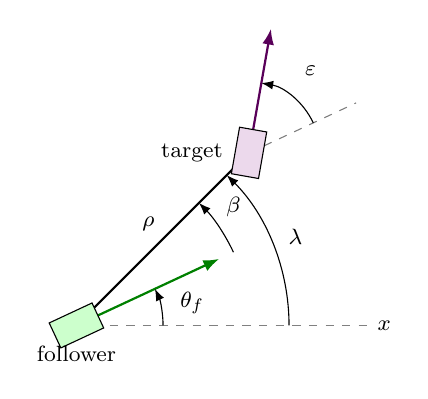
\begin{tikzpicture}[font=\footnotesize]
  \coordinate (F) at (0,0);
  \coordinate (T) at (45:3.1);
  \draw[gray, dashed] (F) -- (3.7,0) node[right, black] {$x$};
  \draw[gray, dashed] (T) -- ++(25:1.5);
  \draw[thick] (F) -- (T) node[midway, above left=-1pt] {$\rho$};
  \draw[-{Latex[length=2mm]}, thick, green!50!black] (F) -- ++(25:2.0);
  \draw[-{Latex[length=2mm]}, thick, violet!70!black] (T) -- ++(80:1.6);
  \node[draw, fill=green!20, rotate=25, minimum width=6mm, minimum height=3.5mm] at (F) {};
  \node[draw, fill=violet!15, rotate=80, minimum width=6mm, minimum height=3.5mm] at (T) {};
  \node[below=4pt] at (F) {follower};
  \node[left=6pt] at (T) {target};
  \draw[-{Latex[length=1.5mm]}] (1.1,0) arc (0:25:1.1);
  \node at (11:1.5) {$\theta_f$};
  \draw[-{Latex[length=1.5mm]}] (2.7,0) arc (0:45:2.7);
  \node at (22:3.0) {$\lambda$};
  \draw[-{Latex[length=1.5mm]}] (25:2.2) arc (25:45:2.2);
  \node at (37:2.5) {$\beta$};
  \draw[-{Latex[length=1.5mm]}, shift={(T)}] (25:0.9) arc (25:80:0.9);
  \node at ($(T)+(53:1.3)$) {$\varepsilon$};
\end{tikzpicture}
\caption{Relative geometry (green: follower, violet: target; arrows show velocity vectors): range $\rho$, bearing $\beta=\lambda-\theta_f$, relative heading $\varepsilon=\theta_t-\theta_f$.}
\label{fig:geom}
\end{figure}

\subsection{Linearization and Local LTI Model}
\label{sec:linearization}

To linearize the model, the nominal straight-line operating condition, where both rovers are moving in the same direction at the same speed while maintaining a constant separation, is considered with:
\[
\rho=d^\ast,\qquad
\beta=\varepsilon=0,\qquad
v_f=v_t=v_0>0,\qquad
\omega_f=\omega_t=0,
\]
where $d^\ast$ is the desired minimal separation between both vehicles and $v_0$ is the nominal forward speed.

The state vector, control input, disturbance from the target's motion, and measured output are then defined as
\[
\mathbf{x}=
\begin{bmatrix}
\delta\rho & \beta & \varepsilon
\end{bmatrix}^{\mathsf T},
\qquad
\mathbf{u}=
\begin{bmatrix}
\delta v_f & \omega_f
\end{bmatrix}^{\mathsf T},
\qquad
\mathbf{w}=
\begin{bmatrix}
\delta v_t & \omega_t
\end{bmatrix}^{\mathsf T},
\]
and
\[
\mathbf{y}=
\begin{bmatrix}
\hat{\rho}-d^\ast\\
\hat{\beta}
\end{bmatrix},
\]
where $\delta\rho=\rho-d^\ast$, $\delta v_f=v_f-v_0$, and $\delta v_t=v_t-v_0$. The relative heading is $\varepsilon=\theta_t-\theta_f$, and the bearing is $\beta=\lambda-\theta_f$. 

The measured outputs are the estimated range deviation $\hat{\delta\rho}$ and relative bearing $\hat{\beta}$ expressed relative to the follower's forward direction.

The control inputs are virtual commands: $\delta v_f$ represents a deviation from the nominal follower speed, while $\omega_f$ represents the commanded follower yaw rate. The target-motion variables $\delta v_t$ and $\omega_t$ are treated as disturbances because the follower does not directly know the target's real-time speed and yaw rate. \autoref{tab:model_variables} showcases the state space variables, their physical interpretation, and associated units. 

Linearizing the nonlinear relative-kinematics model about the nominal operating condition gives
\begin{equation}
\dot{\mathbf{x}}
=\mathbf{A}\mathbf{x}
+\mathbf{B}\mathbf{u}
+\mathbf{E}\mathbf{w},
\qquad
\mathbf{y}
=\mathbf{C}\mathbf{x}+\mathbf{n},
\label{eq:lin}
\end{equation}
where $\mathbf{n}$ represents measurement-estimation errors (to be determined experimentally). The measurement equation applies when a valid acoustic estimate becomes available; measurements are not assumed to arrive at every controller update.

For the constant-speed operating condition, the local model is LTI:
\begin{equation}
\begin{aligned}
\mathbf{A}
&=
\begin{bmatrix}
0&0&0\\
0&0&a\\
0&0&0
\end{bmatrix},
&
\mathbf{B}
&=
\begin{bmatrix}
-1&0\\
0&-1\\
0&-1
\end{bmatrix},\\[6pt]
\mathbf{E}
&=
\begin{bmatrix}
1&0\\
0&0\\
0&1
\end{bmatrix},
&
\mathbf{C}
&=
\begin{bmatrix}
1&0&0\\
0&1&0
\end{bmatrix},
\end{aligned}
\label{eq:mats}
\end{equation}
with
\[
a=\frac{v_0}{d^\ast}.
\]


Refer to Appendix \ref{app:der} for the supplementary derivations and to \autoref{fig:ctrl} for the block diagram. 

\begin{table*}[!t]
\centering
\caption{State-space variables and their physical interpretation.}
\label{tab:model_variables}
\small
\renewcommand{\arraystretch}{1.15}
\begin{tabular}{p{0.15\textwidth} p{0.10\textwidth} p{0.55\textwidth} p{0.10\textwidth}}
\hline
\textbf{Category} & \textbf{Variable} & \textbf{Physical meaning} & \textbf{Unit}\\
\hline
State
& $\delta\rho$
& Deviation of the actual follower-target distance  from the desired separation $d^\ast$
& m\\

State
& $\beta$
& Relative bearing of the target measured from the follower's forward direction
& rad\\

State
& $\varepsilon$
& Relative heading between the target and follower
& rad\\

Control input
& $\delta v_f$
& Deviation of the follower's forward speed from the nominal speed $v_0$
& m/s\\

Control input
& $\omega_f$
& Commanded yaw rate of the follower
& rad/s\\

Disturbance
& $\delta v_t$
& Deviation of the target's forward speed from the nominal speed $v_0$
& m/s\\

Disturbance
& $\omega_t$
& Target's yaw rate
& rad/s\\

Measured output
& $\hat{\rho}-d^\ast$
& Estimated range deviation obtained from the acoustic measurements
& m\\

Measured output
& $\hat{\beta}$
& Estimated relative bearing obtained from the acoustic measurements
& rad\\
\hline
\end{tabular}
\end{table*}

The range estimate is obtained from the amplitude model rather than from a direct distance measurement (\autoref{eq:rho}). 

A discrete-time observer will therefore be considered to estimate the state vector from measurements and control inputs. It will be designed using the discretized local model and will be corrected only when valid acoustic measurements arrive. 

The nonlinear relative-kinematics equations in \autoref{sec:kinematic} will be retained for simulation, while the linearized model will be used for the initial controller design and analysis.

\begin{figure}[!t]
\centering
\resizebox{\linewidth}{!}{%
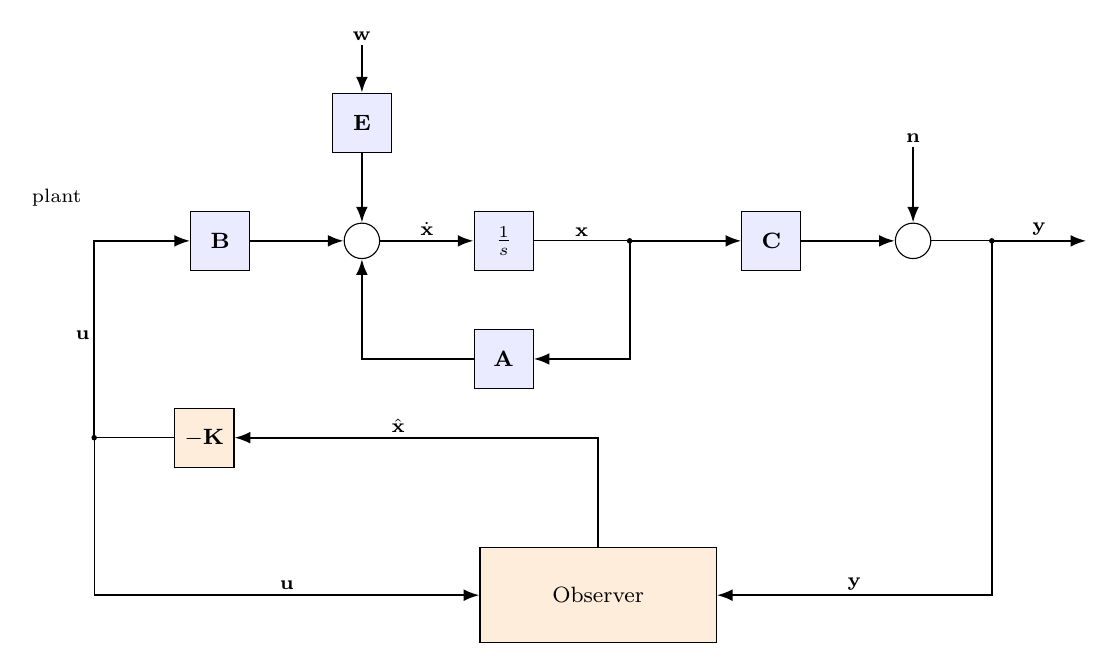
\begin{tikzpicture}[
  font=\footnotesize,
  sq/.style={draw, minimum size=7.5mm, inner sep=1pt, fill=blue!8},
  sqo/.style={draw, minimum size=7.5mm, inner sep=1pt, fill=orange!14},
  sm/.style={circle, draw, inner sep=0pt, minimum size=4.5mm},
  arr/.style={-{Latex[length=2mm]}, thick},
  lbl/.style={font=\scriptsize, inner sep=1.5pt, align=center}
]
% ================= plant =================
\node[sq] (B)  at (1.2,0)  {$\mathbf B$};
\node[sm] (S1) at (3.0,0)  {};
\node[sq] (I)  at (4.8,0)  {$\tfrac1s$};
\coordinate (xd) at (6.4,0);
\node[sq] (C)  at (8.2,0)  {$\mathbf C$};
\node[sm] (S2) at (10.0,0) {};
\node[sq] (E)  at (3.0,1.5) {$\mathbf E$};
\node[sq] (A)  at (4.8,-1.5) {$\mathbf A$};
\node[lbl] (w) at (3.0,2.6) {$\mathbf w$};
\node[lbl] (n) at (10.0,1.3) {$\mathbf n$};
\node[lbl, anchor=east] at (-0.5,0.55) {plant};
% ================= observer and controller =================
\node[sqo, minimum width=30mm, minimum height=12mm] (O) at (6.0,-4.5) {Observer};
\node[sqo] (K) at (1.0,-2.5) {$-\mathbf K$};

% ---- plant wiring
\draw[arr] (B) -- (S1);
\draw[arr] (w) -- (E);
\draw[arr] (E) -- (S1);
\draw[arr] (S1) -- node[above, lbl] {$\dot{\mathbf x}$} (I);
\draw (I) -- node[above, lbl] {$\mathbf x$} (xd);
\fill (xd) circle (1pt);
\draw[arr] (xd) -- (C);
\draw[arr] (xd) -- (6.4,-1.5) -- (A.east);
\draw[arr] (A.west) -- (3.0,-1.5) -- (S1.south);
\draw[arr] (C) -- (S2);
\draw[arr] (n) -- (S2);
\draw (S2.east) -- (11.0,0);
\fill (11.0,0) circle (1pt);
\draw[arr] (11.0,0) -- node[above, lbl] {$\mathbf y$} (12.2,0);
% ---- observer inputs: y and u
\draw[arr] (11.0,0) -- (11.0,-4.5) -- node[above, lbl] {$\mathbf y$} (O.east);
\draw[arr] (-0.4,-4.5) -- node[above, lbl] {$\mathbf u$} (O.west);
% ---- estimate to controller
\draw[arr] (O.north) -- (6.0,-2.5) -- node[above, lbl, pos=0.55] {$\hat{\mathbf x}$} (K.east);
% ---- controller output u to plant and observer
\draw (K.west) -- (-0.4,-2.5);
\fill (-0.4,-2.5) circle (1pt);
\draw[arr] (-0.4,-2.5) -- (-0.4,0) -- (B.west);
\draw (-0.4,-2.5) -- (-0.4,-4.5);
\node[lbl, anchor=east] at (-0.4,-1.2) {$\mathbf u$};
\end{tikzpicture}%
}
\caption{State-space block diagram of the control loop. Blue: Plant components. Orange: Controller and observer blocks.}
\label{fig:ctrl}
\end{figure}

\section{Control Objectives}
\label{sec:control}

Table~\ref{tab:spec} lists the objectives. All numbers are tentative until further testing. Other objectives such as total pursuit time may be added at a later stage based on hardware experiments (\autoref{sec:hardexp}). The rationale for each objective is as follows.

\begin{table}[t!]
\caption{Control and estimation objectives (tentative)}
\label{tab:spec}
\centering
\footnotesize
\renewcommand{\arraystretch}{1.15}
\begin{tabular}{@{}l p{2.1cm} p{5.0cm}@{}}
\toprule
ID & Objective & Target \\
\midrule
O1 & Range regulation & Zero steady-state error to constant $\delta v_t$ \\
O2 & Bearing regulation & RMS $|\beta|\le10^\circ$ (static target), $\le20^\circ$ (moving) \\
O3 & Transient & 2\% settling $\le6\,\mathrm{s}$; overshoot $\le15\%$ \\
O4 & Safety & $\rho\ge\rho_{\min}$; calibrated steering and speed limits respected \\
O5 & Robustness & PM $\ge45^\circ$, GM $\ge6\,\mathrm{dB}$ with delay $T_d$ \\
\bottomrule
\end{tabular}
\end{table}

\begin{itemize}
    \item \textbf{O1, range regulation.} If the target holds a constant speed
    different from the follower's nominal speed ($\delta v_t$ constant), the
    range error must converge to zero. This is achieved by integral action on
    the range error. The guarantee applies to the \emph{estimated} range; a
    calibration error in $K$ would leave a constant offset in the true range.
    \item \textbf{O2, bearing regulation.} The $10^\circ$ static target is attainable. The looser $20^\circ$ moving target allows for the bearing lead that a turning target requires.
    \item \textbf{O3, transient.} The tentative targets are a 2\% settling time of at most $6\,\mathrm{s}$ and overshoot below $15\%$. The achievable response depends on the measured sensing and actuation delay $T_d$. After measuring this delay, the controller bandwidth and gains will be selected through simulation and validated on the physical rovers.
    \item \textbf{O4, safety.} The minimum separation $\rho_{\min}$ will be selected based on the rover geometry, experimentally measured stopping distance, and an appropriate safety margin. Steering and speed commands will be limited to their calibrated operating ranges.
    \item \textbf{O5, robustness.} A phase margin of $45^\circ$ and a gain margin of $6\,\mathrm{dB}$ are standard margins against unmodeled delay and gain error, with the delay $T_d$ the dominant uncertainty.
\end{itemize}

\section{Testing and Validation of the Control Design}
\label{sec:valid}

The general validation approach is to test each part separately (simulation, sensing on the bench, estimation, then the closed loop) before testing them together.

\subsection{Simulation (MATLAB/Simulink and Python)}
The simulated plant is the nonlinear model \eqref{eq:nl} and the acoustic measurement is generated from \eqref{eq:amp}. The estimator and controller are first designed on the linear model in MATLAB and then reimplemented in Python (language used on the Raspberry Pi).
\begin{itemize}
    \item \textbf{Linearization check:} compare the responses of the nonlinear model \eqref{eq:nl} and the linear model \eqref{eq:lin} to initial offsets to find the region in which the linear design can be trusted.
    \item \textbf{Controllability and observability:} compute the controllability and observability matrices and the Gramian condition for different $v_0/d^\ast$.
    \item \textbf{Closed-loop runs:} simulate runs with random initial range and bearing offsets (within the region found in S1) and different noise realizations, and report the average and spread of the settling time, overshoot, and RMS errors.
\end{itemize}

\subsection{Hardware Experiments}
\label{sec:hardexp}
The hardware experiments are listed in Table~\ref{tab:exp}. The first two test the sensing and estimation alone, and the last two close the loop. Reference values come from distances and angles marked on the floor and measured with a tape measure.

\begin{table}[t!]
\caption{Planned hardware experiments}
\label{tab:exp}
\centering
\footnotesize
\renewcommand{\arraystretch}{1.15}
\begin{tabular}{@{}l p{3.7cm} p{2.6cm}@{}}
\toprule
ID & Scenario & Output \\
\midrule
1 & Target at several known angles and distances, follower fixed & $\hat\beta,\hat\rho$ error; fit of $K,\sigma$ \\
2 & Follower fixed (arm only), target driven along a marked path & $\hat\rho,\hat\beta,\hat\varepsilon$ vs.\ reference \\
3 & Closed-loop following of a target moving at constant speed on a straight path & Settling, overshoot, range and bearing error \\
4 & Closed-loop catch-up: follower starts farther than $d^\ast$ from a slowly moving target & Time to reach the separation interval \\
\bottomrule
\end{tabular}
\end{table}

\subsection{Metrics and Acceptance}
The main metrics are the RMS errors of $\rho$ and $\beta$, the 2\% settling time, and the overshoot. The gain and phase margins are computed in MATLAB on the linear model with the measured delay (using Pad\'e approximation). The results are compared with the control objectives O1--O5 of Table~\ref{tab:spec}, first in simulation and then on the hardware. Because the reference measurements are limited to the accuracy of human measurements (using the tape), the hardware errors are expected to be larger than the simulated ones.

\section{Work Plan, Risks and Mitigation}
\label{sec:plan}

\subsection{Work Plan}
The final deliverables are a working demonstration of the follower tracking the target, the simulation and testing results described in Sec.~\ref{sec:valid}, the final report, and the code and data in the project repository. The work plan in the coming weeks is as follows.
\begin{itemize}
    \item \textbf{Weeks 1--2.} Finish the hardware setup. Develop the firmware and start fitting the sensor parameters $K$ and $\sigma$ at the chosen $f_0$. Measure the servo settling time, the measurement delay $T_d$, and the basic vehicle parameters (steering and speed limits, actuator time constants).
    \item \textbf{Weeks 3--4.} Build the simulation of Sec.~\ref{sec:valid}, check the linearization and the controllability and observability analysis numerically, and tune the controller and observer gains.
    \item \textbf{Weeks 5--6.} Run the estimator on real measurements with the target moving, then run the controller on the Raspberry Pi and attempt the first closed-loop following.
    \item \textbf{Weeks 7--8.} Repeat the closed-loop tests, compare the state-feedback controller with the bearing-only baseline, analyze the data against the objectives, and write the final report.
\end{itemize}

\subsection{Risks and Mitigation}
Risks related to the limited accuracy of the range from amplitude are foreseen. The amplitude depends on the speaker level, and an error in $K$ shifts the estimated range. Ti mitigate this risk, a stable supply for the speaker will be used, and $K$ will be recalibrated before each test session.

In addition, the servo dwell time limits the update rate and increases the delay, which limits the achievable bandwidth of the loop. Once the delay is measured and found to be too large, a two-horn configuration can be adopted.

While the Raspberry Pi is not a real-time system, the ESP32 and Pi must exchange data reliably using timestamped measurements and a fixed control rate.

Without a motion-capture system, the reference values come from marked distances and angles, which limits their accuracy. Alternatively, an IMU can be used as ground truth for odometry. 

% ==========================================
% IEEE Standard Bibliography Environment
\bibliographystyle{IEEEtranN}
\bibliography{refs}

\appendices
\section{Repository}
The project repository is available at \href{https://github.com/helenejabbour/Audio-Tracking-Rover}{Audio Tracking Rover}. The final package should include the MATLAB/Simulink model, Python analysis scripts, raw CSV logs, and associated plots and figures.

\section{Supplementary Derivations}
\label{app:der}

\subsection{Linearization}
Let $f_1=v_t\cos\alpha-v_f\cos\beta$, $f_2=(v_t\sin\alpha+v_f\sin\beta)/\rho-\omega_f$, $f_3=\omega_t-\omega_f$. At the nominal point ($\alpha=\beta=0$, $\rho=d^\ast$, $v_t=v_f=v_0$): $\partial f_1/\partial v_t=1$, $\partial f_1/\partial v_f=-1$, with all other partials of $f_1$ zero; $\partial f_2/\partial\alpha=\partial f_2/\partial\beta=v_0/d^\ast=a$, $\partial f_2/\partial\omega_f=-1$, all other partials zero. Using $\alpha+\beta=\varepsilon$ gives $\delta f_2=a\varepsilon-\omega_f$, which yields \eqref{eq:mats}.

\subsection{Estimator Variance}
From \eqref{eq:beta}, $\partial\hat\beta/\partial\ln A_\pm=\pm\sigma^{2}/(2\delta)$, so $\operatorname{var}\hat\beta=2(\sigma^{2}/2\delta)^{2}\sigma_{\ln A}^{2}$. For fixed additive noise $\sigma_n$, $\sigma_{\ln A}=\sigma_n/A_\pm=(\sigma_n/A_{pk})e^{\delta^{2}/2\sigma^{2}}$, hence $\sigma_\beta\propto e^{\delta^{2}/2\sigma^{2}}/\delta$, minimized at $\delta=\sigma$. From \eqref{eq:rho}, $\ln\hat\rho=\ln K-\tfrac12(\ln A_++\ln A_-)+\text{const}$, so $\operatorname{var}(\ln\hat\rho)=\sigma_{\ln A}^{2}/2$.

\section{Proof of Concept}
\label{app:poc}
A proof of concept (POC) was conducted to evaluate the extent to which the MAX4466 microphone can detect a change in distance or orientation of the emitted sound. 

\begin{figure}[ht!]
\begin{center}
    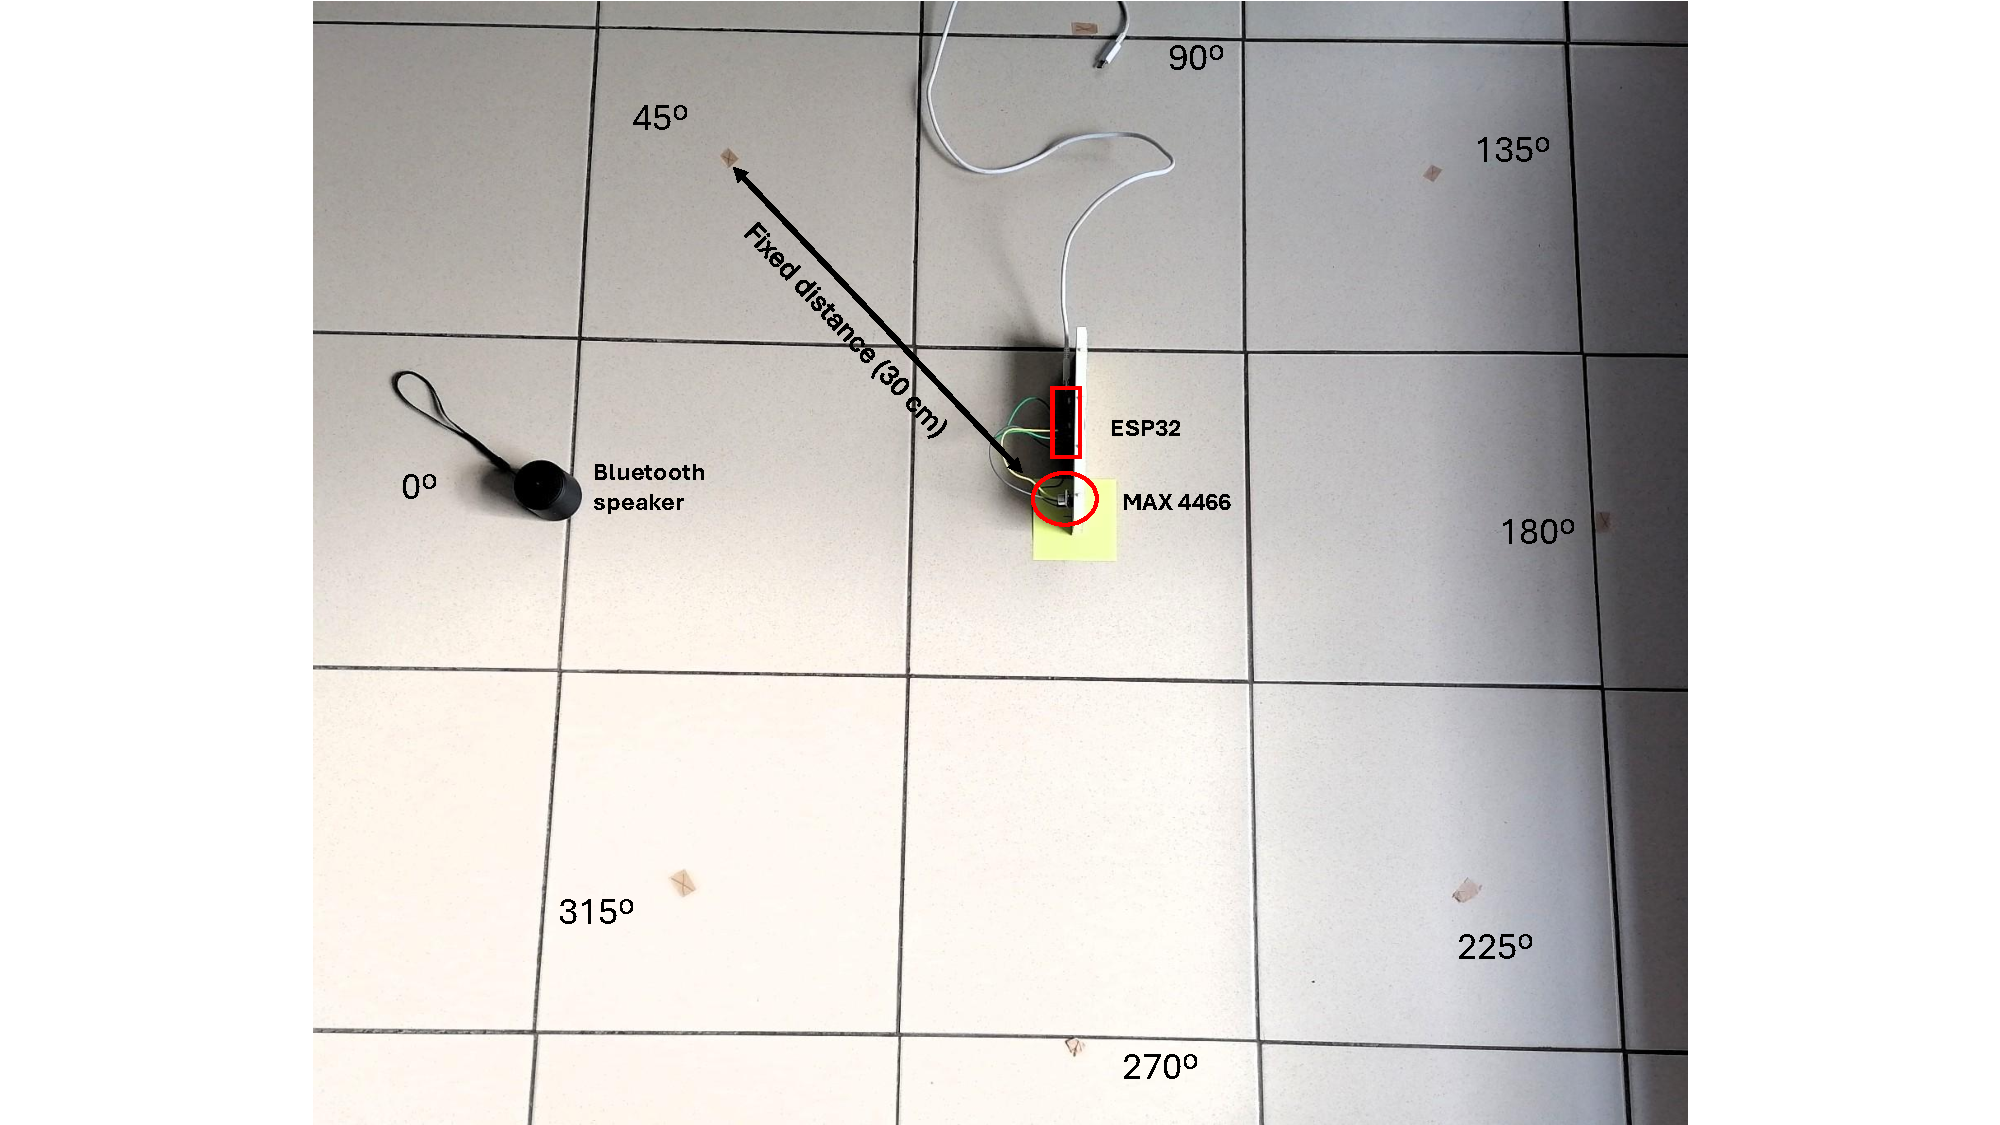
\includegraphics[width=0.7\linewidth]{poc.pdf}
    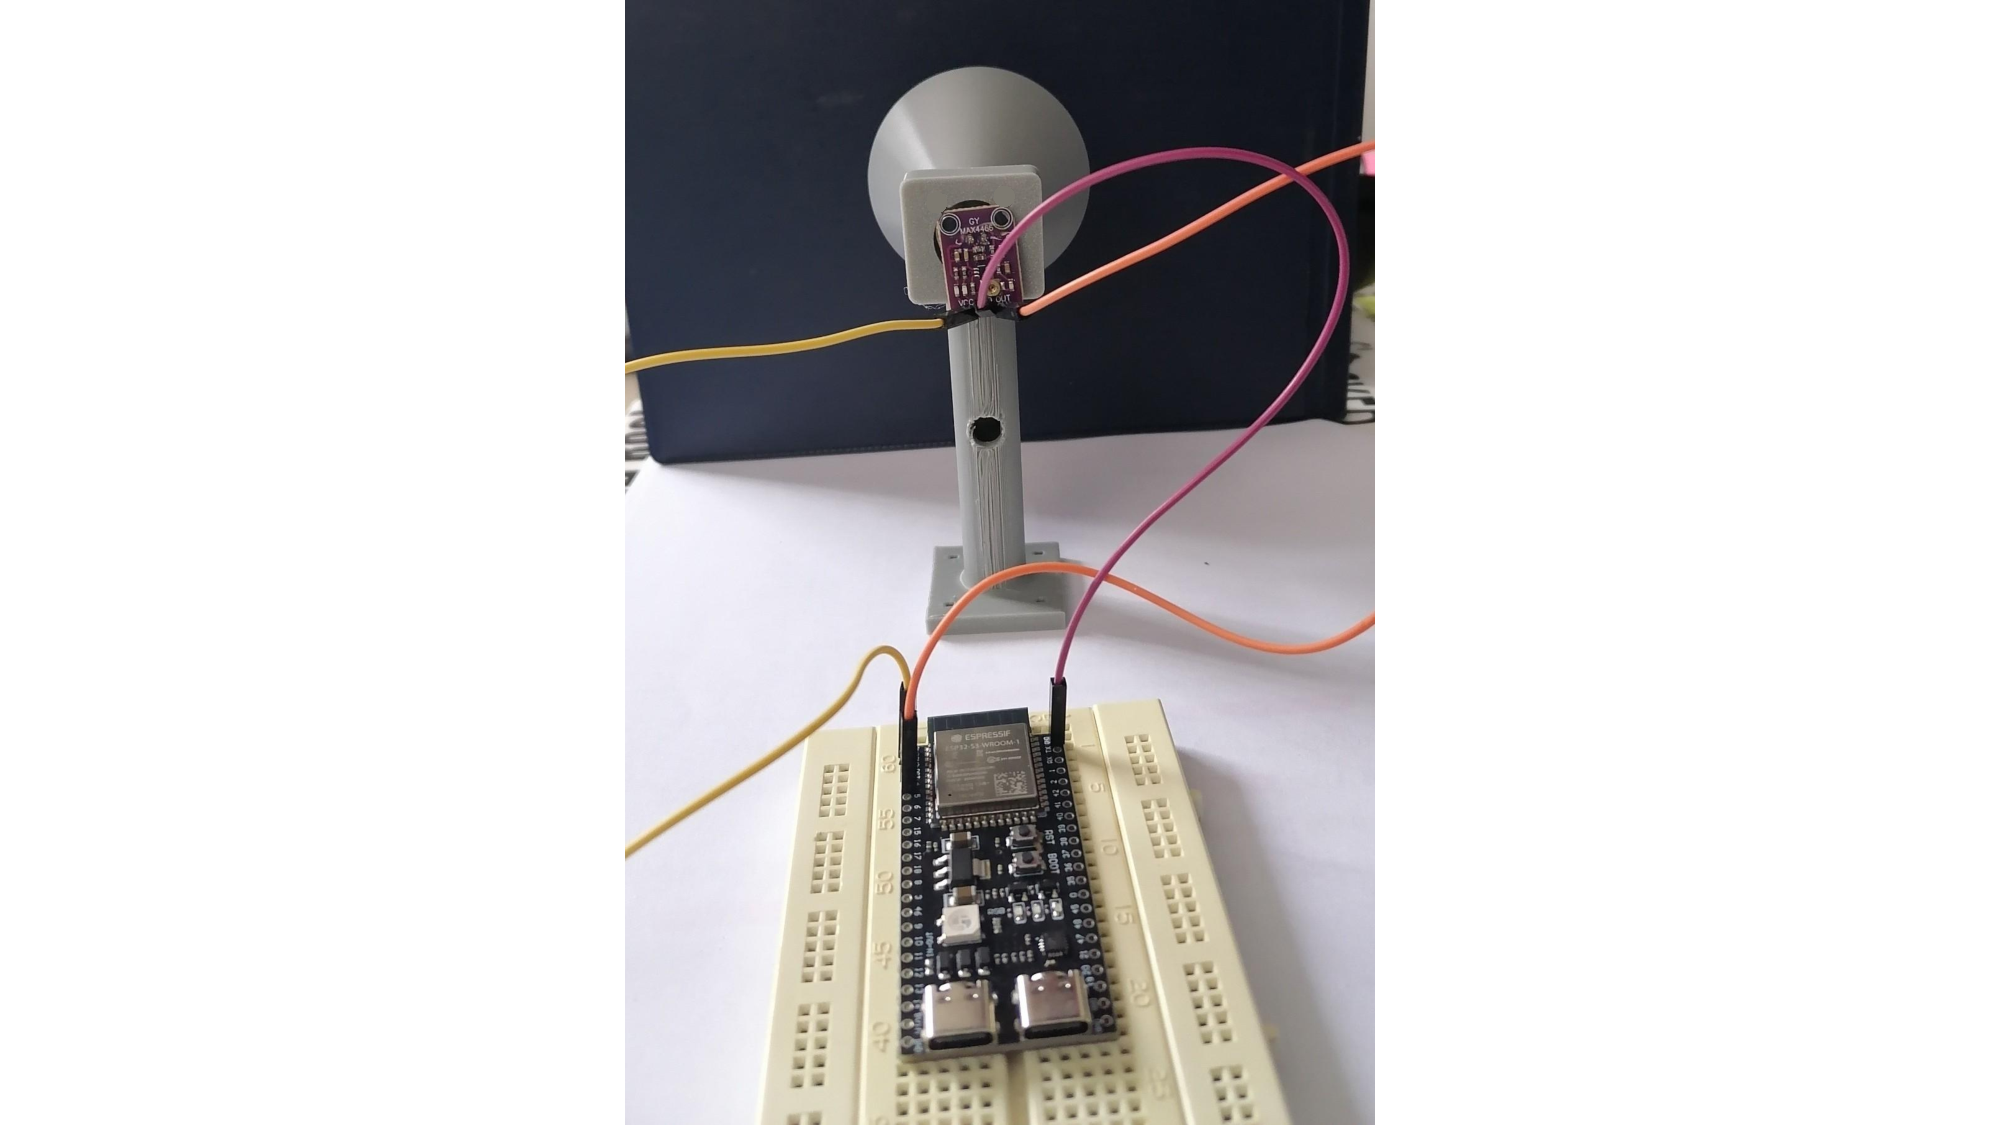
\includegraphics[width=0.2\linewidth]{mic_horn.pdf}
    \caption{Setup of the proof of concept including MAX 4466, ESP32, a breadboard, and a speaker with no horn (left) and zoom-in on the microphone + horn mounting for the second stage of the proof of concept (right).}
    \label{fig:poc}
\end{center}
\end{figure}

In the first stage, the microphone was connected to an ESP32 on a breadboard and placed at a fixed point, while a Bluetooth speaker was alternating across $8$ angular positions at a fixed distance of $30\text{ cm}$ (\autoref{fig:poc} left). The sound emitted consisted of a ``chirp'' at a constant frequency and regular intervals. Each angle sweep, at repeated measurements, exhibited peak-to-trough differences of approximately $5.2\text{--}7.8\text{ dB}$. The minimum amplitude was consistently recorded at $180^\circ$, while the maximum occurred near $0^\circ$ at around $63.0\text{ dB}$. Between $0^\circ$ and $180^\circ$, a drop of about $2\text{ dB}$ per $45^\circ$ was observed, with a symmetric behavior between $180^\circ$ and $360^\circ$ (\autoref{fig:polarplot} left). These results indicate the dependence of the response amplitude on the orientation of the sound source.

In the second stage, the same experiment was repeated with the 3D-printed directional horn attached to the microphone (\autoref{fig:poc} right). All other testing conditions were exactly the same. The results showed similar findings to the first stage of POC, but the signal level was approximately $2\text{ dB}$ higher in the horn pointing direction between $0^\circ\text{--}45^\circ$ and $315^\circ\text{--}360^\circ$, reaching approximately $65.0\text{ dB}$. This corresponds to a peak-to-trough difference of $10.3\text{--}10.5\text{ dB}$ (\autoref{fig:polarplot} right). This difference is higher than that recorded in the first stage, suggesting that the horn increases contrast of the measured signal between orientations. Therefore, these findings support the potential use of the horn in the assembly, although further testing at smaller angular increments is needed to achieve better sensitivity.

\begin{figure}[ht!]
\begin{center}
    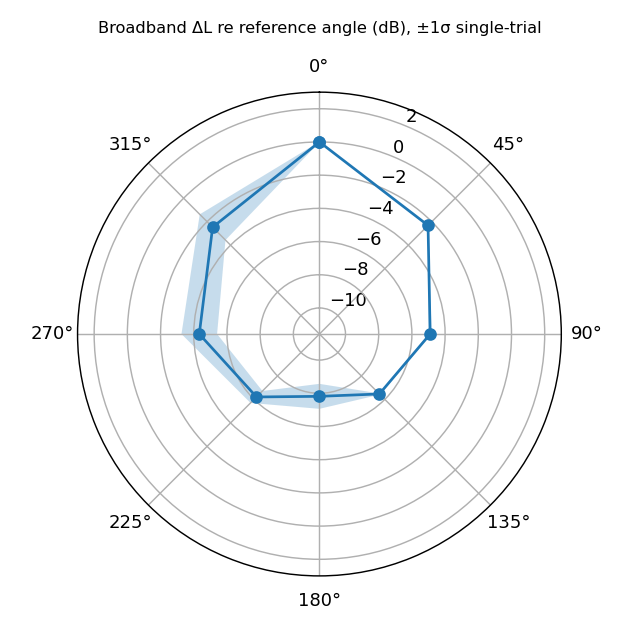
\includegraphics[width=0.43\linewidth]{bare1_summary_angle.png}
    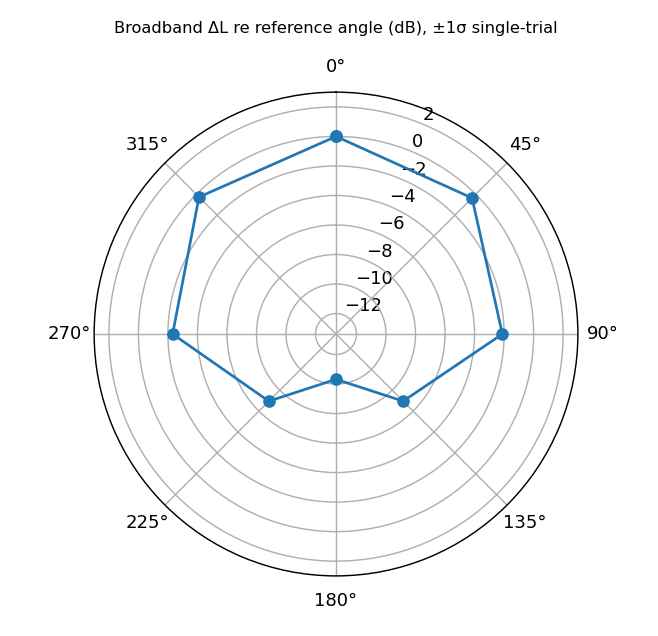
\includegraphics[width=0.43\linewidth]{horn1_summary_angle.png}
    \caption{\textbf{Measured directional gain profiles of the acoustic receiver setup.} Broadband relative sound level $\Delta L$ (dB) with respect to reference angle ($0^\circ$), evaluated across 8 angular increments ($45^\circ$ steps). \textbf{Left:} Baseline microphone setup without the directional horn. \textbf{Right:} Comparative profile with the 3D-printed directional horn.}
    \label{fig:polarplot}
\end{center}
\end{figure}

\section{Model Assumptions}
The key modeling assumptions along with their purpose are presented in the table below.
\begin{table}[H]
\centering
\caption{Key modeling assumptions.}
\label{tab:model_assumptions}
\small
\renewcommand{\arraystretch}{1.2}
\begin{tabular}{p{0.3\linewidth} p{0.65\linewidth}}
\hline
\textbf{Assumption} & \textbf{Purpose} \\
\hline
Horn response as Gaussian
& Enables closed-form bearing estimation from two acoustic amplitudes. \\

Inverse-distance amplitude response
& Enables local range estimation from acoustic amplitude. \\

Target motion limited during a measurement pair
& Reduces errors caused by measuring the two amplitudes at different times. \\

Local linear approximation
& Supports state-feedback design using a tractable state-space model. \\

Actuator mapping is sufficiently accurate
& Connects virtual speed and yaw-rate inputs to the physical rover commands. \\
\hline
\end{tabular}
\end{table}


\end{document}
